\section{Prospetto economico}
In questa sezione è presentato il prospetto economico del progetto MaaS, suddiviso per fasi. Il costo è calcolato utilizzando i dati
riportati nei \textit{Vincoli sull’organigramma del gruppo e sull’offerta tecnico-economica}:
\href{http://www.math.unipd.it/~tullio/IS-1/2015/Progetto/PD01b.html}{http://www.math.unipd.it/~tullio/IS-1/2015/Progetto/PD01b.html}


%-----------------------------------------------------------------------------------------------------
%-------------------------------------- ANALISI ------------------------------------------------------
%-----------------------------------------------------------------------------------------------------
\subsection{Analisi}
A scopo di trasparenza viene redatto il prospetto economico riguardante la fase di Analisi dei Requisiti, che si precisa essere a carico del fornitore, e non del proponente.

\begin{table}[H]
	\centering
	\begin{tabular}{ l c c }
		\textbf{Ruolo} & \textbf{Ore} & \textbf{Costo} \\
		\hline
		Amministratore & 33 & 600 \euro \\
		Analista & 50 & 1250 \euro \\
		Progettista & 8 & 176 \euro \\
		Programmatore & 0 & 0 \euro \\
		Responsabile & 33 & 990 \euro \\
		Verificatore & 36 & 540 \euro \\
		\hline
		Totale & 160 & 3556 \euro \\
		\hline
	\end{tabular}
	\caption{Ore e costo per ruolo, periodo di Analisi}
\end{table}

I seguenti grafici mostrano il peso orario e di costo di ogni ruolo in questo periodo.

\begin{figure}[H]
  \begin{center}
    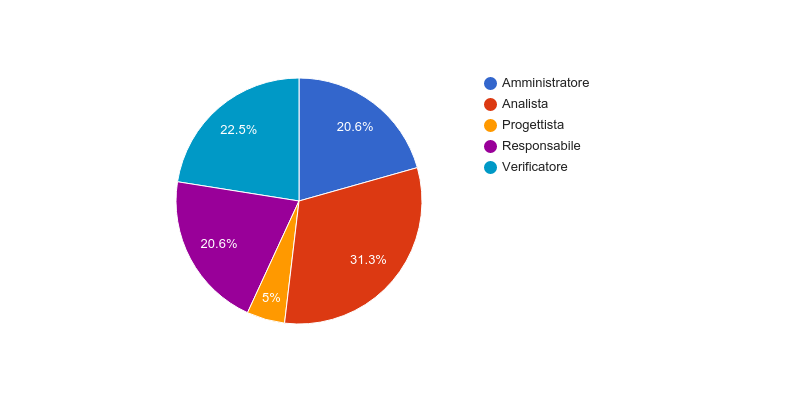
\includegraphics[width=12cm]{res/img/orePerRuoloAnalisi.png}
  \caption{Ore per componente, fase di Analisi}
  \end{center} 
\end{figure}  

\begin{figure}[H]
  \begin{center}
    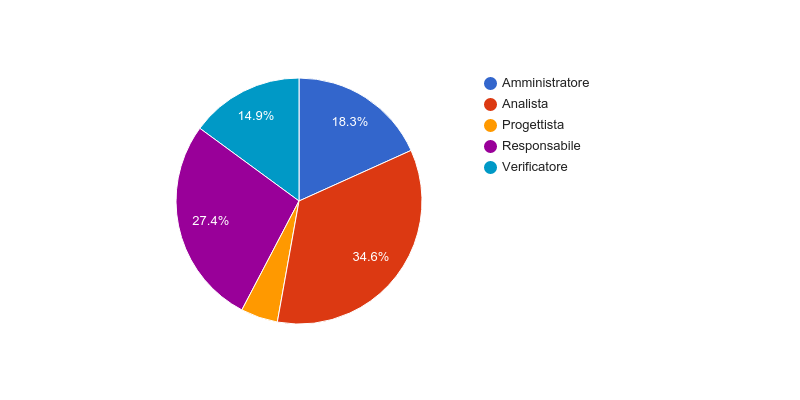
\includegraphics[width=12cm]{res/img/costoPerRuoloAnalisi.png}
  \caption{Costo per ruolo, fase di Analisi}
  \end{center} 
\end{figure}  


%-----------------------------------------------------------------------------------------------------
%-------------------------------------- ANALISI MIGLIORAMENTI ----------------------------------------
%-----------------------------------------------------------------------------------------------------
\subsection{Analisi Miglioramenti}
A scopo di trasparenza viene redatto il prospetto economico riguardante la fase di Analisi Miglioramenti.

\begin{table}[H]
	\centering
	\begin{tabular}{ l c c }
		\textbf{Ruolo} & \textbf{Ore} & \textbf{Costo} \\
		\hline
		Amministratore & 11 & 220 \euro \\
		Analista & 4 & 100 \euro \\
		Progettista & 3 & 66 \euro \\
		Programmatore & 0 & 0 \euro \\
		Responsabile & 1 & 30 \euro \\
		Verificatore & 11 & 165 \euro \\
		\hline
		Totale & 30 & 581 \euro \\
		\hline
	\end{tabular}
	\caption{Ore e costo per ruolo, periodo di Analisi}
\end{table}

I seguenti grafici mostrano il peso orario e di costo di ogni ruolo in questo periodo.

\begin{figure}[H]
  \begin{center}
    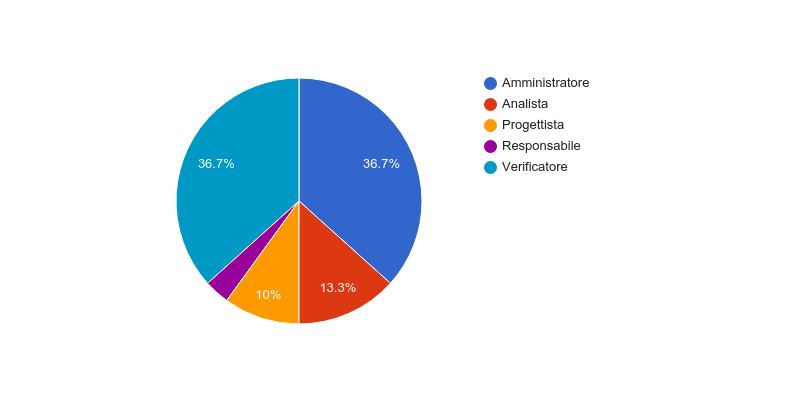
\includegraphics[width=12cm]{res/img/orePerRuoloAnalisiMiglioramenti.png}
  \caption{Ore per componente, fase di Analisi}
  \end{center} 
\end{figure}  

\begin{figure}[H]
  \begin{center}
    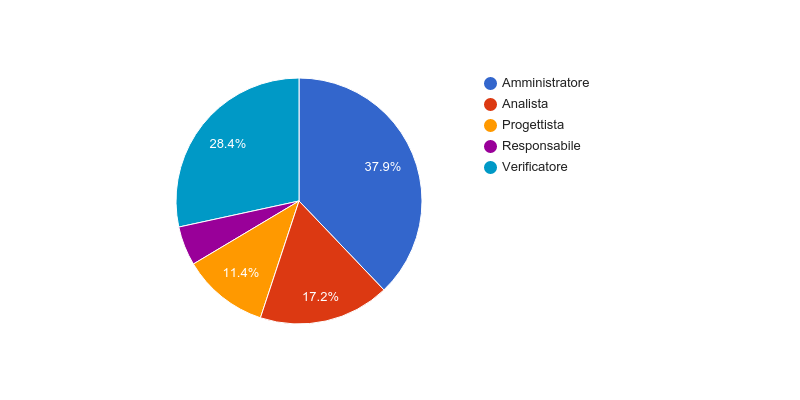
\includegraphics[width=12cm]{res/img/costoPerRuoloAnalisiMiglioramenti.png}
  \caption{Costo per ruolo, fase di Analisi}
  \end{center} 
\end{figure}  


%-----------------------------------------------------------------------------------------------------
%-------------------------------------- PROGETTAZIONE ARCHITETTURALE ---------------------------------
%-----------------------------------------------------------------------------------------------------
\subsection{Progettazione Architetturale}
Nella fase di Progettazione Architetturale le ore per ogni ruolo sono state cos\`i suddivise:

\begin{table}[H]
	\centering
	\begin{tabular}{ l c c }
		\textbf{Ruolo} & \textbf{Ore} & \textbf{Costo} \\
		\hline
		Amministratore & 8 & 160 \euro \\
		Analista & 3 & 75 \euro \\
		Progettista & 141 & 3102 \euro \\
		Programmatore & 0 & 0 \euro \\
		Responsabile & 2 & 60 \euro \\
		Verificatore & 74 & 1110 \euro \\
		\hline
		Totale & 228 & 4507 \euro \\
		\hline
	\end{tabular}
	\caption{Ore e costo per ruolo, periodo di Progettazione Architetturale}
\end{table}

I seguenti grafici mostrano il peso orario e di costo di ogni ruolo in questo periodo.

\begin{figure}[H]
  \begin{center}
    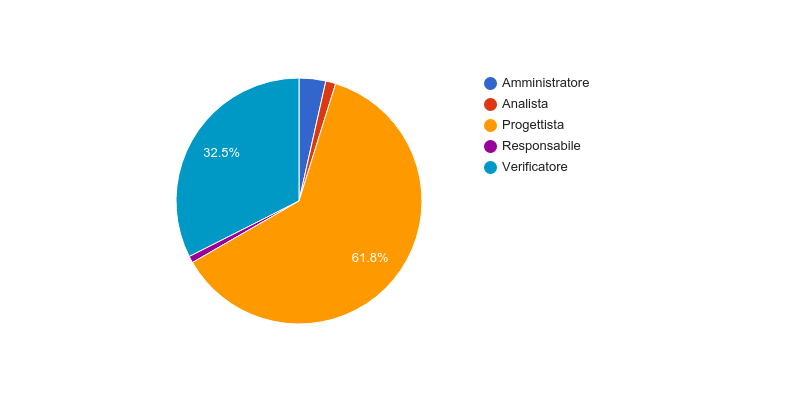
\includegraphics[width=12cm]{res/img/orePerRuoloProgettazioneArchitetturale.png}
  \caption{Ore per componente, fase di Progettazione Architetturale}
  \end{center} 
\end{figure}  

\begin{figure}[H]
  \begin{center}
    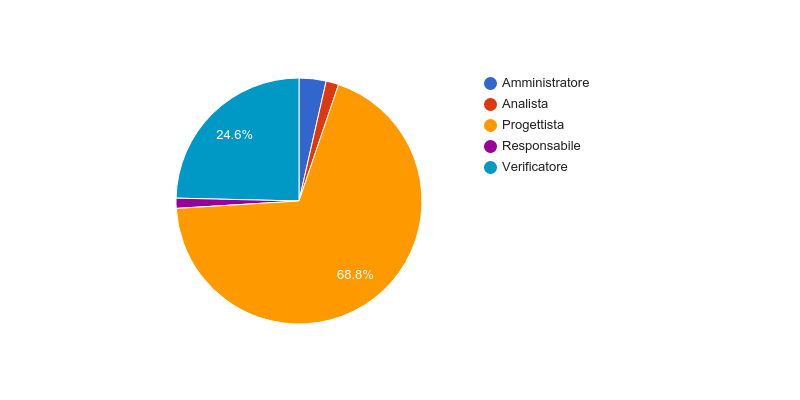
\includegraphics[width=12cm]{res/img/costoPerRuoloProgettazioneArchitetturale.png}
  \caption{Costo per ruolo, fase di Progettazione Architetturale}
  \end{center} 
\end{figure}  


%-----------------------------------------------------------------------------------------------------
%-------------------------------------- PROGETTAZIONE DI DETTAGLIO E CODIFICA ------------------------
%-----------------------------------------------------------------------------------------------------
\subsection{Progettazione di dettaglio e codifica}
Nel periodo di Progettazione di Dettaglio e Codifica le ore per ogni ruolo sono state così suddivise:

\begin{table}[H]
	\centering
	\begin{tabular}{ l c c }
		\textbf{Ruolo} & \textbf{Ore} & \textbf{Costo} \\
		\hline
		Amministratore & 50 & 1000 \euro \\
		Analista & 3 & 75 \euro \\
		Progettista & 120 & 2640 \euro \\
		Programmatore & 138 & 2070 \euro \\
		Responsabile & 3 & 90 \euro \\
		Verificatore & 54 & 810 \euro \\
		\hline
		Totale & 368 & 6685 \euro \\
		\hline
	\end{tabular}
	\caption{Ore e costo per ruolo, periodo di Progettazione di Dettaglio e Codifica}
\end{table}

I seguenti grafici mostrano il peso orario e di costo di ogni ruolo in questo periodo.

\begin{figure}[H]
  \begin{center}
    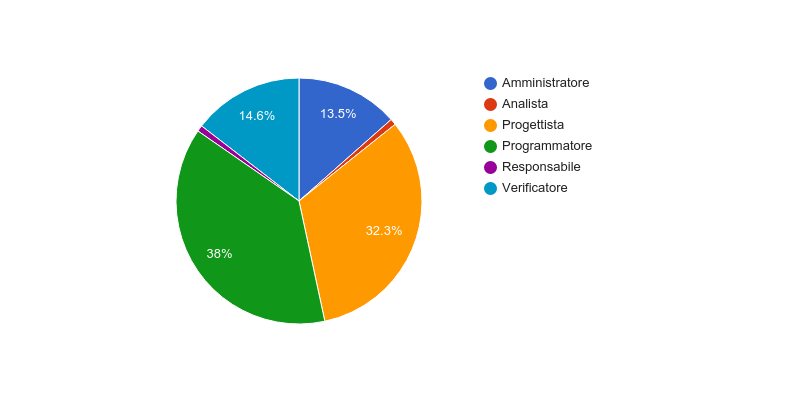
\includegraphics[width=12cm]{res/img/orePerRuoloProgettazioneDettaglioCodifica.png}
  \caption{Ore per componente, fase di Progettazione di Dettaglio e Codifica}
  \end{center} 
\end{figure}  

\begin{figure}[H]
  \begin{center}
    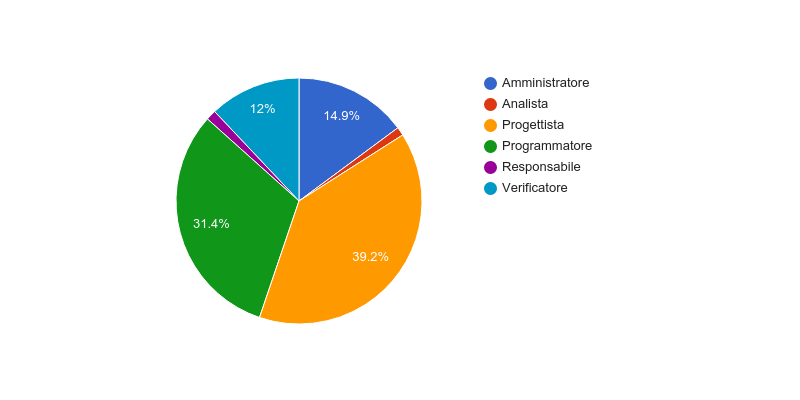
\includegraphics[width=12cm]{res/img/costoPerRuoloProgettazioneDettaglioCodifica.png}
  \caption{Costo per ruolo, fase di Progettazione di Dettaglio e Codifica}
  \end{center} 
\end{figure}  


%-----------------------------------------------------------------------------------------------------
%-------------------------------------- VERIFICA E VALIDAZIONE ---------------------------------------
%-----------------------------------------------------------------------------------------------------
\subsection{Verifica e Validazione}
Nel periodo di Validazione le ore per ogni ruolo sono state cosi suddivise:

\begin{table}[H]
	\centering
	\begin{tabular}{ l c c }
		\textbf{Ruolo} & \textbf{Ore} & \textbf{Costo} \\
		\hline
		Amministratore & 13 & 260 \euro \\
		Analista & 0 & 0 \euro \\
		Progettista & 12 & 264 \euro \\
		Programmatore & 5 & 75 \euro \\
		Responsabile & 6 & 180 \euro \\
		Verificatore & 70 & 1050 \euro \\
		\hline
		Totale & 106 & 1829 \euro \\
		\hline
	\end{tabular}
	\caption{Ore e costo per ruolo, periodo di Validazione}
\end{table}

I seguenti grafici mostrano il peso orario e di costo di ogni ruolo in questo periodo.

\begin{figure}[H]
  \begin{center}
    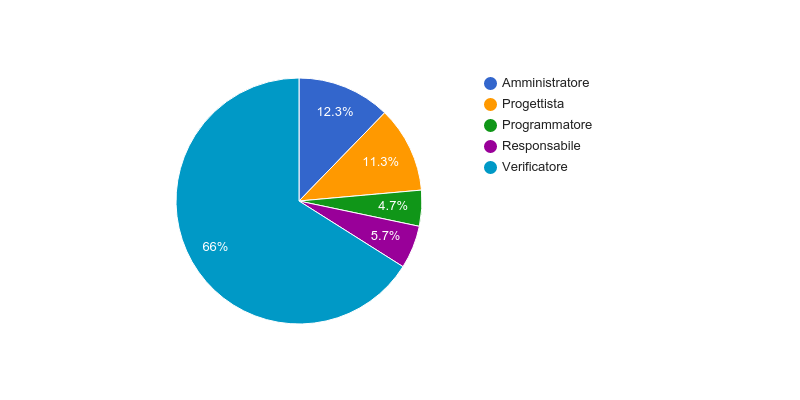
\includegraphics[width=12cm]{res/img/orePerRuoloValidazione.png}
  \caption{Ore per componente, fase di Validazione}
  \end{center} 
\end{figure}  

\begin{figure}[H]
  \begin{center}
    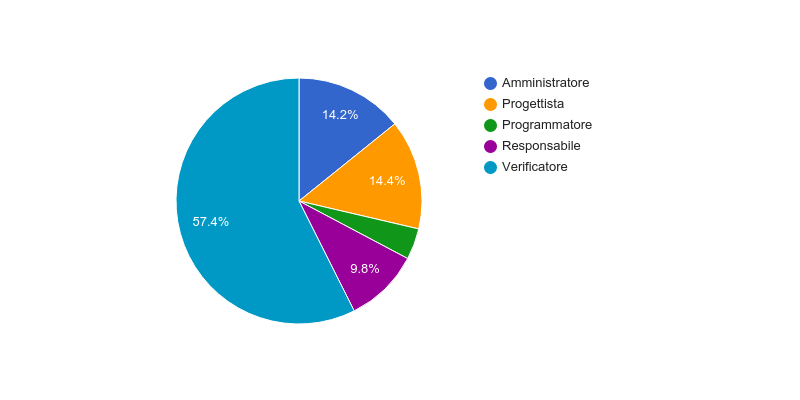
\includegraphics[width=12cm]{res/img/costoPerRuoloValidazione.png}
  \caption{Costo per ruolo, fase di Validazione}
  \end{center} 
\end{figure}  


%-----------------------------------------------------------------------------------------------------
%-------------------------------------- TOTALE -------------------------------------------------------
%-----------------------------------------------------------------------------------------------------
\subsection{Totale}
In totale le ore per ogni ruolo sono state così suddivise:

\begin{table}[H]
	\centering
	\begin{tabular}{ l c c }
		\textbf{Ruolo} & \textbf{Ore} & \textbf{Costo} \\
		\hline
		Amministratore & 115 & 2300 \euro \\
		Analista & 60 & 1500 \euro \\
		Progettista & 284 & 6248 \euro \\
		Programmatore & 143 & 2145 \euro \\
		Responsabile & 45 & 1350 \euro \\
		Verificatore & 245 & 3675 \euro \\
		\hline
		Totale & 892 & 0 \euro \\
		\hline
	\end{tabular}
	\caption{Ore e costo per ruolo, riassunto progetto}
\end{table}

Il seguente grafico mostra il costo di ogni ruolo durante tutto lo svolgimento del progetto, escluso il periodo di Analisi dei Requisiti.

\begin{figure}[H]
  \begin{center}
    \includegraphics[width=12cm]{res/img/orePerRuoloRiassuntoProgetto.png}
  \caption{Ore per componente, riassunto progetto}
  \end{center} 
\end{figure}  

\begin{figure}[H]
  \begin{center}
    \includegraphics[width=12cm]{res/img/costoPerRuoloRiassuntoProgetto.png}
  \caption{Costo per ruolo, riassunto progetto}
  \end{center} 
\end{figure}  


Ricordando che le ore di Analisi dei requisiti sono a carico del fornitore le ore totali per ogni ruolo sono state così suddivise:
\begin{table}[H]
	\centering
	\begin{tabular}{ l c c }
		\textbf{Ruolo} & \textbf{Ore} & \textbf{Costo} \\
		\hline
		Amministratore & 115 & 2300 \euro \\
		Analista & 60 & 1500 \euro \\
		Progettista & 284 & 6248 \euro \\
		Programmatore & 143 & 2145 \euro \\
		Responsabile & 45 & 1350 \euro \\
		Verificatore & 245 & 3675 \euro \\
		\hline
		Totale & 892 & 0 \euro \\
		\hline
	\end{tabular}
	\caption{Ore e costo per ruolo, riassunto progetto}
\end{table}

Il seguente grafico mostra il costo di ogni ruolo durante tutto lo svolgimento del progetto.

\begin{figure}[H]
  \begin{center}
    \includegraphics[width=12cm]{res/img/orePerRuoloRiassuntoProgetto.png}
  \caption{Ore per componente, riassunto progetto}
  \end{center} 
\end{figure}  

\begin{figure}[H]
  \begin{center}
    \includegraphics[width=12cm]{res/img/costoPerRuoloRiassuntoProgetto.png}
  \caption{Costo per ruolo, riassunto progetto}
  \end{center} 
\end{figure}  

